\documentclass{ximera}

\input{../preamble.tex}



\title{8.8 - The Fundamental Theorem of Calculus (Part 2)}

\begin{document}
\begin{abstract}
The accumulation of a rate is given by the change in quantity.
\end{abstract}
\maketitle

There is a another common form of the Fundamental Theorem of Calculus:

\begin{theorem}[Fundamental Theorem of Calculus (Part 2)]\index{Second Fundamental Theorem of Calculus}
  Let $f$ be continuous on $[a,b]$. If $F$ is \textbf{any}
  antiderivative of $f$, then
  \[
  \int_a^b f(x)\d x = F(b)-F(a).
  \]
  \begin{explanation}
    Let $a\le c\le b$ and write
    \begin{align*}
      \int_a^b f(x) \d x &= \int_a^c f(x) \d x + \int_c^b f(x) \d x \\
      &= \int_c^b f(x) \d x - \int_c^a f(x) \d x.
    \end{align*}
    By the First Fundamental Theorem of Calculus, we have
    \[
    F(b) = \int_c^b f(x) \d x\qquad\text{and}\qquad F(a) = \int_c^a f(x) \d x
    \] 
    for some antiderivative $F$ of $f$. So
    \[
    \int_a^b f(x) \d x = F(b)-F(a)
    \]
    for this antiderivative. However, \textbf{any} antiderivative
    could have be chosen, as antiderivatives of a given function
    differ only by a constant, and this constant \textit{always}
    cancels out of the expression when evaluating $F(b)-F(a)$.
\end{explanation}
\end{theorem}

%From this you should see that the two versions of the Fundamental Theorem are very closely related. 
While the two parts of the Fundamental Theorem of Calculus look different at first, they are actually deeply related. In fact, the two forms are
\textbf{equivalent}, just differently stated. %Hence people often simply call them both ``The Fundamental Theorem of Calculus.''
One way of thinking about the Fundamental Theorem of Calculus (Part 2) is the following:
\begin{image}
  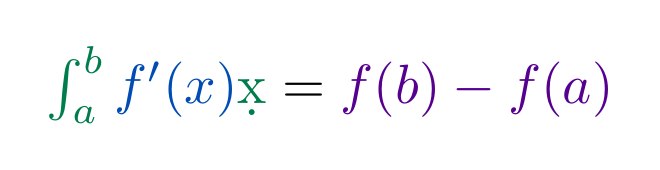
\begin{tikzpicture}[scale=2,every node/.style={transform shape}]
    \node at (0,0) {
      $\color{green!70!black!70!blue}\int_a^b\color{blue!70!green}f'(x)\color{green!70!black!70!blue}\d x\color{black} = 
      \color{purple!50!blue!90!black}f(b) - f(a)$
      };
  \end{tikzpicture}
\end{image}
This could be read as:
\begin{quote}\large\textbf{The \textcolor{green!70!black!70!blue}{accumulation} of a \textcolor{blue!70!green}{rate} is given by the \textcolor{purple!50!blue!90!black}{change in quantity}.}
\end{quote}



Using this version of the Fundamental Theorem, when we compute a definite integral, we first find an antiderivative
and then evaluate at the limits of integration and subtract. It is convenient to
first display the antiderivative and then evaluate.  A special
notation is often used in the process of evaluating definite integrals
using the Fundamental Theorem of Calculus. Instead of explicitly
writing $F(b)-F(a)$, we often write
\[
F(x)\Bigr\vert_a^b \mbox{  or  } \eval{F(x)}_a^b
\]
meaning that one should evaluate $F(x)$ at $b$ and then subtract
$F(x)$ evaluated at $a$:
\[
F(x)\Bigr\vert_a^b =\eval{F(x)}_a^b= F(b)-F(a).
\]

Let's see some examples of the fundamental theorem in action.

\begin{example}
  Compute:
  \[
  \int_{-2}^2 x^3\d x
  \]
  \begin{explanation}
    We start by finding an antiderivative of $x^3$. The simplest choice is $\frac{1}{4}x^{4}$. Hence
    \begin{align*}
      \int_{-2}^2 x^3 \d x &=\frac{1}{4}x^4\Bigr\vert_{-2}^2\\
      &= \frac{1}{4}(2)^4 - \frac{1}{4}(-2)^4\\
      &= 0.
    \end{align*}
  \end{explanation}
\end{example}


\begin{example}
  Compute:
  \[
  \int_0^\pi \sin \theta \d \theta
  \]
  \begin{explanation}
    We start by finding an antiderivative of $\sin \theta$. The simplest choice is $-\cos\theta$. Hence
    \begin{align*}
      \int_0^\pi \sin\theta \d \theta &= \eval{-\cos\theta}_0^{\pi}\\
      &=\answer[given]{-\cos(\pi)} - (-\cos(0))\\
      &=\answer[given]{2}.
    \end{align*}
    This is interesting: It says that the area under one ``hump'' of a
    sine curve is $2$.
  \end{explanation}
\end{example}

\begin{example}
  Compute:
  \[
  \int_0^5 e^t\d t
  \]
  \begin{explanation}
    We start by finding an antiderivative of $e^t$. The simplest choice is $\answer[given]{e^t}$. Hence
    \begin{align*}
      \int_0^5 e^t \d t &= e^t\biggr\vert_0^5 \\
      &= e^5-\answer[given]{e^0}\\
      &= e^5-\answer[given]{1}.
    \end{align*}
  \end{explanation}
\end{example}


\begin{example}
Compute:
\[
\int_1^2\left(x^9 + \frac{1}{x}\right) \d x
\]
\begin{explanation}
We start by finding an antiderivative of $x^9 + \frac{1}{x}$. The simplest choice is $\frac{x^{10}}{10} + \ln(x)$. Hence
\begin{align*}
\int_1^2\left(x^9 + \frac{1}{x}\right) \d x &= \left(\frac{x^{10}}{10} + \ln(x)\right)\biggr\vert_1^2 \\
&= \frac{2^{10}}{10} + \ln(2) - \answer[given]{\frac{1}{10}}.
\end{align*}
\end{explanation}
\end{example}




%\section{Understanding motion with the Fundamental Theorem of Calculus}
%
%We know that
%\begin{itemize}
%\item The derivative of a position function is a velocity function.
%\item The derivative of a velocity function is an acceleration
%  function.
%\end{itemize}
%Now consider definite integrals of velocity and acceleration
%functions. Specifically, if $v(t)$ is a velocity function, what does
%$\int_a^b v(t)\d t$ mean?
%
%The Fundamental Theorem of Calculus (Part 2) states that
%\[
%\int_a^b v(t)\d t = V(b) - V(a),
%\]
%where $V(t)$ is any antiderivative of $v(t)$. Since $v(t)$ is a
%velocity function, $V(t)$ must be a position function, and $V(b) -
%V(a)$ measures a \textbf{change in position}, or \dfn{displacement}.
%
%\begin{example}
%  A ball is thrown straight up with velocity given by $v(t) =
%  -32t+20$ft/s, where $t$ is measured in seconds. Find, and interpret,
%  $\int_0^1 v(t)\d t$.
%    \begin{explanation}
%      Using the Fundamental Theorem of Calculus, we have
%      \begin{align*}
%        \int_0^1 v(t)\d t &= \int_0^1 (-32t+20)\d t \\
%	&= \left(\answer[given]{-16t^2 + 20t}\right)\biggr\vert_0^1 \\
%	&=[-16(1)^2+20(1)]-[-16(0)^2+20(0)]\\
%	&= 4.
%      \end{align*}
%      Thus if a ball is thrown straight up into the air with velocity
%      \[
%      v(t) = \answer[given]{-32t+20},
%      \]
%      the height of the ball, $1$ second later, will be $4$ feet above the
%      initial height. Note that the ball has \textit{traveled} much
%      farther. It has gone up to its peak and is falling down, but the
%      difference between its height at $t=0$ and $t=1$ is $4$ft. 
%    \end{explanation}
%\end{example}    



Now we know that to compute a definite integral,  we ``merely'' find an antiderivative, substitute two values, and subtract. Unfortunately, as we have seen,
finding antiderivatives can be quite difficult. While there are a
small number of rules that allow us to compute the derivative of any
common function, there are no such rules for antiderivatives. There
are some techniques that frequently prove useful, but we will never be
able to reduce the problem to a completely mechanical process.



\subsection{Learning Objectives}
After completing this section, students should be able to:
\vspace{.05in}

\noindent$\bullet$ State the Fundamental Theorem of Calculus (Part 2).
\\$\bullet$ Evaluate definite integrals using the Fundamental Theorem of Calculus (Part 2).
\\$\bullet$ Understand how the area under a curve is related to the antiderivative.
\\$\bullet$ Understand the relationship between indefinite and definite integrals.




\end{document}